\documentclass[10pt,a4paper]{article}
\usepackage[top=100pt,bottom=50pt,left=48pt,right=46pt]{geometry}
%Gummi|065|=)

\usepackage{multirow}
\usepackage{amsmath}
\usepackage{makecell}
\usepackage{graphicx}
\usepackage{hyperref}
\usepackage{cite}
\begin{document}
\begin{center}
\LARGE{\textbf{Project Report:}}\\
\LARGE{\textbf{``Prediction of Whether a Player can Score Goal or Not''}}\\[0.5cm]
\vspace{0.8cm}

\Large{\textbf{Submitted by}}
\begin{center}
\begin{tabular}{ c c c }
 Swapnil Biswas & & 14.02.04.021 \\ 
 Shahariar Shibli & & 14.02.04.027\\
 Lab Group - 02 & & Section - A1
\end{tabular}
\end{center}

\vspace{0.8cm}
\Large{\textbf{CSE 4108}}\\
\Large{\textbf{Artificial Intelligence Lab}}\\

\vspace{0.8cm}
\Large{\textbf{Submitted to}}\\[0.4cm]
Mr. Taksir Hasan Majumder\\
Lecturer\\
Department of Computer Science and Engineering

\vspace{0.4cm}
	
Mir Imtiaz Mostafiz\\
Lecturer\\
Department of Computer Science and Engineering\\

\vspace{0.8cm}
\vspace{0.4cm}

\includegraphics[scale=0.25]{LogoAust.jpg}\\
\vspace{0.4cm}
\Large{\textbf{AHSANULLAH UNIVERSITY OF SCIENCE \& TECHNOLOGY}}\\
\vspace{0.8cm}
\today

\vspace{0.5cm}
\end{center}


\newpage

\section{Introduction}
The Game of Football is, without doubt, the most popular game in the world today. The very term, ''football'', has a romance of its own. It is, indeed, a word of millions to conjure with. A good schemer in the forward line is, indeed, a veritable artist. Successful defenders play the game with perfect anticipation, neat tackling, superb head-work and sudden burst of overlapping. A competitive game in progress is, surely, a fascinating treat to watch.\\

\section{Problem Description}
The importance of anything depends on who is participating in the activity. Therefore, players scoring goals for a team in a particular match is very essential. In this project, we have tried to predict whether a player can score at least 1 goal or not based on some relevant information. But we have worked with a small dataset which consists of only 102 instances.

\section{Dataset Description}
\begin{itemize}
    \item The dataset contains information that we have collected to predict whether a football player can score a goal or not in a match. The data are obtained from~\cite{a}.
    
    \item Dataset contains 102 instances and prediction is done based on 2 classes which are represented by 0 and 1. 0 indicates the player doesn't score any goal and 1 indicates that the player scores in a particular match.
    
    \item Class 0 contains 58 instances and class 1 contains 44 instances. No attribute has missing values.
    
    \item In total 9 attributes are used such as - Name, Player's Current Rating, Age, Recent Form, Position, Opponent Team's Rating, Own Team's Rating, Venue and Target.
    
    \item Player's current rating describes the performance of the player in that particular match. Recent Form of a player is the number of goals scored by him till now in this season.
    
    \item Venue is divided into 2 classes represented by 1 and 2. 1 is for Home match \& 2 is for Away match. Also, position of a player is categorized only into three classes represented by 1,2 \& 3. 1 is for Froward, 2 is for Midfield \& 3 is for Defense.  
    
    \item The information of players and teams we have collected to create the dataset is based on the season 2017/2018.
\end{itemize}

\section{Feature Selection}
We have computed correlation between the attributes and we have found that we can simply ignore the attribute 'Venue' that effects the prediction less.

\section{Description of the Models}
We have used 5 models in this problem to see which one gives the better accuracy. As we have used K-Fold Cross Validation with k=5 dataset is divided into 5 folds and 4 folds are used for training purpose and the rest 1 is used for testing purpose. So, 80\% data is used for training and the rest 20\% is used for testing.Then, different classifiers used different slices exactly 5 times and we kept lists to keep the results for each.

\subsection{Decision Tree Classifier}
\textbf{}Decision Tree is a type of Supervised Machine Learning Method where the data is continuously split according to a certain parameter. It breaks down a data set into smaller and smaller subsets while at the same time an associated decision tree is incrementally developed. The tree can be explained by two entities, namely decision nodes and leaves. The leaves are the decisions or the final outcomes. And the decision nodes are where the data is split.\\
\begin{figure}[]
\centering
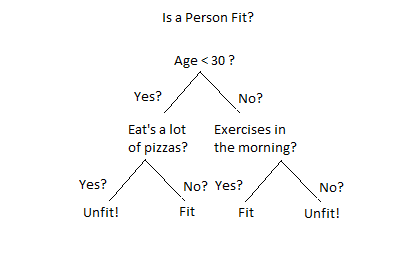
\includegraphics[scale=1.00]{Decision-Trees.png}
\caption{Example of Decision Tree~\cite{a}}
\end{figure}\\
An example of a decision tree can be explained using above binary tree. Let’s say we want to predict whether a person is fit given their information like age, eating habit, and physical activity, etc. The decision nodes here are questions like ‘What’s the age?’, ‘Does he exercise?’, ‘Does he eat a lot of pizzas’? And the leaves, which are outcomes like either ‘fit’, or ‘unfit’. In this case this is a binary classification problem (a 'yes' 'no' type problem).

\subsection{Gaussian Naive Bayes Classifier}
The Naive Bayesian classifier is based on Bayes’ theorem with independence assumptions between predictors. A Naive Bayesian model is easy to build, with no complicated iterative parameter estimation which makes it particularly useful for very large data sets. Despite its simplicity, the Naive Bayesian classifier often does surprisingly well and is widely used because it often outperforms more sophisticated classification methods.\\\\
When attribute values are continuous, an assumption is made that the values associated with each class are distributed according to Gaussian i.e., Normal Distribution.
\begin{figure}[htp]
\centering
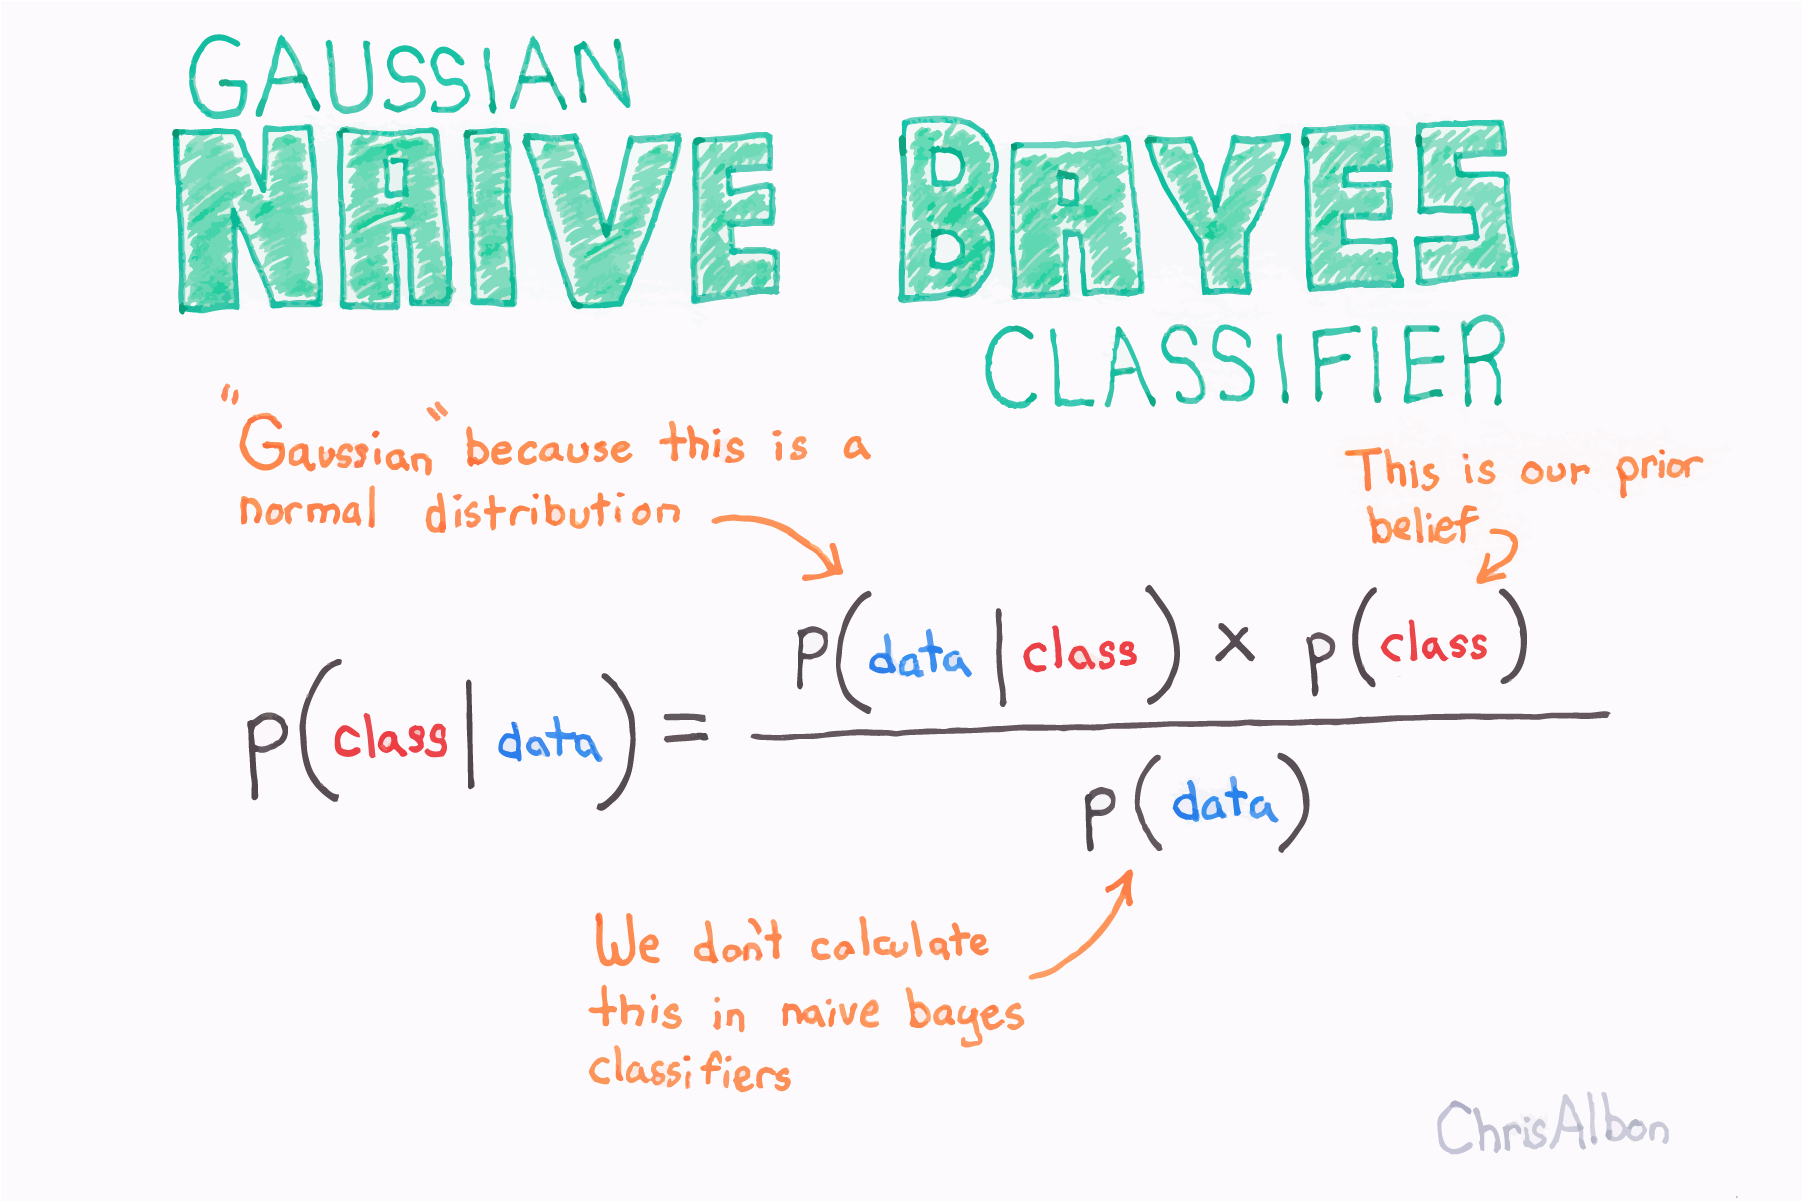
\includegraphics[scale=0.90]{Gaussian_Naive_Bayes_Classifier_print.png}
\caption{Gaussian Naive Bayes Probability Equation~\cite{b}}
\end{figure}\\

\subsection{Random Forest Classifier}
\textbf{Random forest classifier} is an ensemble algorithm. Random forest classifier creates a set of decision trees from randomly selected subset of training set. It then aggregates the votes from different decision trees to decide the final class of the test object. Let’s look into a real life example to understand the random forest algorithm.\\\\
Suppose Shuvo somehow got 2 weeks leave from his office. He wants to spend his 2 weeks by traveling to the different place. He also wants to go to the place he may like.So he decided to ask his best friend about the places he may like. Then his friend started asking about his past trips. It’s just like his best friend will ask, You have been visited the X place did you like it?\\\\
To recommend the best place to Shuvo, his best friend asked some questions. Based on the answers given by Shuvo, he recommended a place. This is decision tree algorithm approach.\\\\
As his best friend may recommend his best place to Shuvo as a friend. The model will be biased with the closeness of their friendship. So he decided to ask few more friends to recommend the best place he may like.\\\\
Now his friends asked some random questions and each one recommended one place to Shuvo. Now  Shuvo considered the place which is high votes from his friends as the final place to visit. This is random forest algorithm.
For the above example help is taken from~\cite{c}.

\subsection{K Nearest Neighbour Classifier}
\textbf{}K-Nearest Neighbor (K-NN) is a non-parametric, instance-based classifier. It is used in a variety of applications such as economic forecasting, data compression and genetics. It needs Minimal training but testing is expensive.Let’s take a simple case to understand this algorithm. Following is a spread of red circles (RC) and green squares (GS) :\\
\begin{figure}[htp]
\centering
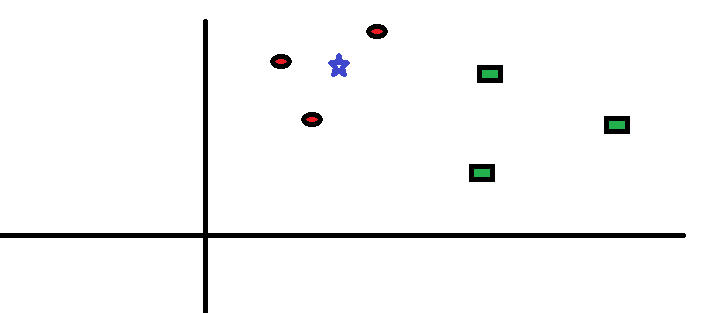
\includegraphics[scale=0.4]{scenario1.png}
\caption{Example of K-NN~\cite{d}}
\end{figure}\\
We intend to find out the class of the blue star (BS) . BS can either be RC or GS and nothing else. The “K” is KNN algorithm is the nearest neighbors we wish to take vote from. Let’s say K = 3. Hence, we will now make a circle with BS as center just as big as to enclose only three data points on the plane. Refer to following diagram for more details:\\
\begin{figure}[htp]
\centering
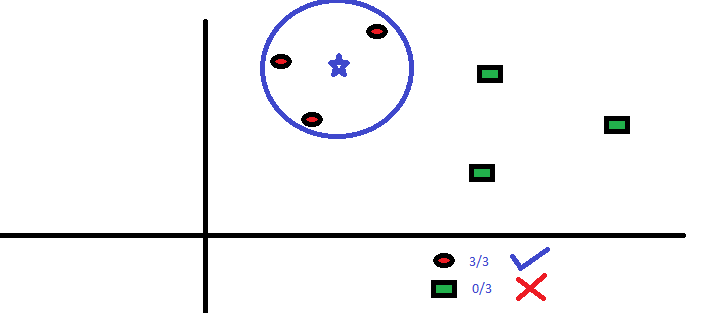
\includegraphics[scale=0.4]{scenario2.png}
\caption{Example of K-NN~\cite{d}}
\end{figure}\\
The three closest points to BS is all RC in figure 4. Hence, with good confidence level we can say that the BS should belong to the class RC. Here, the choice became very obvious as all three votes from the closest neighbor went to RC. To determine which of the K instances in the training dataset are most similar to a new input, a distance measure is used. For real-valued input variables, the most popular distance measure is Euclidean distance. In our code we used this classifer with k=5.
\vspace{1.8cm}
\subsection{AdaBoost Classifier}
\textbf{}AdaBoost is a type of "Ensemble Learning" where multiple learners are employed to build a stronger learning algorithm. AdaBoost works by choosing a base algorithm (e.g. decision trees) and iteratively improving it by accounting for the incorrectly classified examples in the training set.\\\\
We assign equal weights to all the training examples and choose a base algorithm. At each step of iteration, we apply the base algorithm to the training set and increase the weights of the incorrectly classified examples. We iterate n times, each time applying base learner on the training set with updated weights. The final model is the weighted sum of the n learners.\\\\
The essence of adaptive boosting is as follows. For now, let's consider the binary classification case.  This is a super-simplified version that eschews all the maths, but gives the flavor:
\begin{enumerate}
    \item Take your favorite learning algorithm.
    \item Apply it on your data. Say we have 100 examples. You'll get some of the class labels wrong. Say you got it 90 correct, 10 wrong.
    \item Reweight or resample the instances in training set so that your learning algorithm now has an error rate of 50\%. So, for example, you might say something like "I'm going to copy the ones I got wrong 9 times for the next iteration". This makes the data set 90 correct, and 90 incorrect. 
    \item Go back to step 2, but applying it to the new data set from step 3. Keep repeating this process, each time producing a new classifier.
    \item Stop when you (a) have done this enough times (b) you get 100\% accuracy. This gives you, say, 7 different classifiers.
    \item To classify, do a "vote" across all of the learning algorithms you built in steps 2 to 4. 
\end{enumerate}\\
The above procedure is taken from~\cite{e}.

\section{Performance Scores of Models}
\begin{table}[htp]
\centering
\caption{Comparison between different classifiers}
\label{my-label}
\begin{tabular}{|l|l|l|l|l|}
\hline
                                                         & Accuracy       & Precision      & Recall         & F1 Score       \\ \hline
\begin{tabular}[c]{@{}l@{}}Random \\ Forest\end{tabular} & 0.911904761905 & 0.90952020202  & 0.918931068931 & 0.909848096348 \\ \hline
\begin{tabular}[c]{@{}l@{}}Decision \\ Tree\end{tabular} & 0.912380952381 & 0.910984848485 & 0.917502497502 & 0.909197825566 \\ \hline
KNN                                                      & 0.921428571429 & 0.922853535354 & 0.925714285714 & 0.919767605265 \\ \hline
adaBoost                                                 & 0.921428571429 & 0.9275         & 0.91984015984  & 0.918899820486 \\ \hline
GNB                                                      & 0.921428571429 & 0.92557026307        & 0.920879120879  & 0.917578178182 \\ \hline
\end{tabular}
\end{table}

\section{Discussion}
\textbf{}From the comparison table we have seen that the best accuracy we have is 92.14\% by KNN,GNB and adaBoost classifiers though their Precision,Recall and F1 scores are different. However, our dataset is not sufficient, we will collect more data and try to improve prediction accuracy in future.

\bibliography{ref}
\bibliographystyle{unsrt}

\end{document}}

